\documentclass[aspectratio=169,12pt,t]{beamer}

% --- Theme: Metropolis (modern, clean) ---
\usetheme[progressbar=frametitle,numbering=fraction,block=fill]{metropolis}

% --- Fira Sans font (install texlive-fonts-extra if missing) ---
\IfFileExists{FiraSans.sty}{\usepackage[sfdefault]{FiraSans}}{}

% --- Light background with warm accent ---
\definecolor{mDarkTeal}{RGB}{35,55,59}
\definecolor{mLightBrown}{RGB}{235,228,216}
\definecolor{mAccent}{RGB}{140,70,20}

\setbeamercolor{normal text}{fg=mDarkTeal,bg=white}
\setbeamercolor{alerted text}{fg=mAccent}
\setbeamercolor{frametitle}{bg=mDarkTeal,fg=white}
\setbeamercolor{progress bar}{fg=mAccent,bg=mLightBrown}
\setbeamercolor{title separator}{fg=mAccent}
\setbeamercolor{progress bar in head/foot}{fg=mAccent,bg=mLightBrown}
\setbeamercolor{progress bar in section page}{fg=mAccent,bg=mLightBrown}

% --- Packages ---
\usepackage[utf8]{inputenc}
\usepackage{amsmath,amssymb,amsthm}
\usepackage{mathrsfs}
\usepackage{tikz}
\usetikzlibrary{arrows.meta,positioning,calc,decorations.pathreplacing,shapes,patterns}
\usepackage{pgfplots}
\pgfplotsset{compat=1.18}

% --- Custom colors for content types ---
\definecolor{defcolor}{RGB}{25,85,120}
\definecolor{thmcolor}{RGB}{140,35,35}
\definecolor{proofcolor}{RGB}{35,100,50}
\definecolor{excolor}{RGB}{140,75,10}
\definecolor{remcolor}{RGB}{90,90,90}

% --- Beamer blocks for mathematical content types ---
\newenvironment{defblock}[1]{%
  \setbeamercolor{block title}{bg=defcolor,fg=white}%
  \setbeamercolor{block body}{bg=defcolor!5}%
  \begin{block}{#1}}{\end{block}}

\newenvironment{thmblock}[1]{%
  \setbeamercolor{block title}{bg=thmcolor,fg=white}%
  \setbeamercolor{block body}{bg=thmcolor!5}%
  \begin{block}{#1}}{\end{block}}

\newenvironment{proofblock}[1]{%
  \setbeamercolor{block title}{bg=proofcolor,fg=white}%
  \setbeamercolor{block body}{bg=proofcolor!5}%
  \begin{block}{#1}}{\end{block}}

\newenvironment{exblock}[1]{%
  \setbeamercolor{block title}{bg=excolor,fg=white}%
  \setbeamercolor{block body}{bg=excolor!5}%
  \begin{block}{#1}}{\end{block}}

\newenvironment{remblock}[1]{%
  \setbeamercolor{block title}{bg=remcolor,fg=white}%
  \setbeamercolor{block body}{bg=remcolor!5}%
  \begin{block}{#1}}{\end{block}}

% --- Metadata ---
\title{Chapter 1: The Real and Complex Number Systems}
\subtitle{Section: Euclidean Spaces}
\author{Based on Walter Rudin's \emph{Principles of Mathematical Analysis}}
\date{}

\begin{document}

% =============================================================================
% TITLE AND OUTLINE
% =============================================================================

\begin{frame}
  \titlepage
  \note{
    Welcome to Chapter 1, Section 7: Euclidean Spaces. In this section we
    generalize what we have done so far to higher dimensions. We define the
    space "R" "k" of ordered "k"-tuples of real numbers, equip it with an inner
    product and a norm, and prove the fundamental properties of the norm,
    including the Schwarz inequality and the triangle inequality. These
    results will allow us to treat "R" "k" as a metric space, which is the
    starting point for all the topology and analysis in later chapters.
  }
\end{frame}

\begin{frame}{Outline}
  \tableofcontents
  \note{
    Here is our outline for this section. We begin with the definitions of
    "R" "k", its vector operations, the inner product, and the norm. Then we
    state and prove Theorem 1.37, which gives six key properties of the norm.
    The proof relies on the Schwarz inequality from the previous section.
    Finally, we close with some remarks connecting "R" "k" to the metric
    spaces we will study in Chapter 2. Let's get started.
  }
\end{frame}

% =============================================================================
% MOTIVATION
% =============================================================================

\section{Definitions and Setup}

% --- Build 1/3 ---
\begin{frame}{Why Euclidean Spaces?}
  \begin{itemize}
    \item So far: $\mathbb{R}$ (the real line) and $\mathbb{C}$ (the complex plane)
  \end{itemize}

  \note{
    Let's begin with some context. In the previous sections we carefully
    built the real number system and the complex number system. The reals
    give us a complete ordered field, and the complex numbers give us an
    algebraically closed field. But both of these are essentially
    one-dimensional or two-dimensional objects. What if we need more
    dimensions?
  }
\end{frame}

% --- Build 2/3 ---
\begin{frame}{Why Euclidean Spaces?}
  \begin{itemize}
    \item So far: $\mathbb{R}$ (the real line) and $\mathbb{C}$ (the complex plane)
    \item Many applications need \alert{higher dimensions}: physics, geometry, data
  \end{itemize}

  \note{
    In many parts of mathematics and its applications we need to work in
    higher dimensions. Physics uses three-dimensional space, quantum
    mechanics uses infinite-dimensional spaces, and many modern applications
    in data science and optimization work in spaces of very high dimension.
    We need a framework that handles all of these dimensions at once. So
    what is our plan?
  }
\end{frame}

% --- Build 3/3 ---
\begin{frame}{Why Euclidean Spaces?}
  \begin{itemize}
    \item So far: $\mathbb{R}$ (the real line) and $\mathbb{C}$ (the complex plane)
    \item Many applications need \alert{higher dimensions}: physics, geometry, data
    \item Goal: define $\mathbb{R}^k$ with an \alert{inner product} and \alert{norm}, then prove
      key inequalities
  \end{itemize}

  \note{
    Our goal in this section is to define the space "R" "k" for any positive
    integer "k", equip it with an inner product and a norm, and then establish
    the fundamental inequalities --- particularly the triangle inequality ---
    that make "R" "k" into a metric space. Let's start with the definitions.
  }
\end{frame}

% =============================================================================
% DEFINITION 1.36
% =============================================================================

\begin{frame}{Definition 1.36: The Space $\mathbb{R}^k$}
  \begin{defblock}{Definition 1.36: Points and Vectors}
    For each positive integer $k$, let $\mathbb{R}^k$ be the set of all ordered $k$-tuples
    \[
      \mathbf{x} = (x_1, x_2, \dots, x_k),
    \]
    where $x_1, \dots, x_k$ are real numbers, called the \alert{coordinates} of $\mathbf{x}$.
  \end{defblock}

  \vspace{0.5em}
  The elements of $\mathbb{R}^k$ are called \emph{points} or \emph{vectors}.

  \note{
    Here is the basic definition. "R" "k" is the set of all ordered "k"-tuples
    of real numbers. The numbers "x" one through "x" "k" are the coordinates of
    the point "x". We call the elements of "R" "k" either points or vectors,
    depending on the context. When "k" equals 1, this is just the real line.
    When "k" equals 2, this is the plane. When "k" equals 3, this is
    three-dimensional space. But the definition works for any positive
    integer "k". Next, let's define the algebraic operations on these vectors.
  }
\end{frame}

% --- Build 1/2: Addition ---
\begin{frame}{Definition 1.36: Vector Operations}
  Let $\mathbf{x} = (x_1, \dots, x_k)$, $\mathbf{y} = (y_1, \dots, y_k)$, and $\alpha \in \mathbb{R}$.

  \vspace{0.5em}
  \textbf{Addition:}
  \[
    \mathbf{x} + \mathbf{y} = (x_1 + y_1, \dots, x_k + y_k)
  \]

  \note{
    Vector addition is defined component by component: you add the first
    coordinates, the second coordinates, and so on. This is exactly what you
    would expect. Notice that the sum of two vectors in "R" "k" is again a
    vector in "R" "k", so "R" "k" is closed under addition. Now let's see
    scalar multiplication.
  }
\end{frame}

% --- Build 2/2: Scalar multiplication ---
\begin{frame}{Definition 1.36: Vector Operations}
  Let $\mathbf{x} = (x_1, \dots, x_k)$, $\mathbf{y} = (y_1, \dots, y_k)$, and $\alpha \in \mathbb{R}$.

  \vspace{0.5em}
  \textbf{Addition:}
  \[
    \mathbf{x} + \mathbf{y} = (x_1 + y_1, \dots, x_k + y_k)
  \]

  \textbf{Scalar multiplication:}
  \[
    \alpha\mathbf{x} = (\alpha x_1, \dots, \alpha x_k)
  \]

  \note{
    Scalar multiplication scales each coordinate by the real number alpha.
    Again, the result is in "R" "k". Together, addition and scalar multiplication
    satisfy all the usual laws: commutativity, associativity, and
    distributivity. These follow trivially from the corresponding properties
    of the real numbers. This makes "R" "k" a vector space over the real field.
    Let's also note the special zero element.
  }
\end{frame}

\begin{frame}{Definition 1.36: Vector Space Structure}
  With these operations, $\mathbb{R}^k$ is a \alert{vector space over the real field}.

  \vspace{0.5em}
  The \emph{zero element} (also called the \emph{origin} or \emph{null vector}):
  \[
    \mathbf{0} = (0, 0, \dots, 0)
  \]

  \vspace{0.5em}
  \textbf{Key:} All vector space laws (commutativity, associativity, distributivity)
  follow immediately from the corresponding laws for $\mathbb{R}$.

  \note{
    The zero vector is the "k"-tuple with all coordinates equal to zero. It
    serves as the additive identity: adding it to any vector gives back the
    same vector. Notice that verifying the vector space laws here is trivial,
    since everything reduces to the corresponding property of the real numbers
    applied coordinate by coordinate. This is much simpler than the previous
    section, where proving the field axioms for the complex numbers required
    real computation. But the vector space structure alone is just algebra.
    The interesting geometry comes next, from the inner product and the norm.
  }
\end{frame}

% =============================================================================
% INNER PRODUCT AND NORM
% =============================================================================

% --- Build 1/2: Inner product ---
\begin{frame}{Definition 1.36: Inner Product and Norm}
  \textbf{Inner product} (or scalar product) of $\mathbf{x}$ and $\mathbf{y}$:
  \[
    \mathbf{x} \cdot \mathbf{y} = \sum_{i=1}^{k} x_i y_i
  \]

  \note{
    The inner product, also called the scalar product or dot product, takes
    two vectors and produces a single real number. You multiply corresponding
    coordinates and add up the results. As shown in the formula on the slide,
    this is a sum of "k" products. Geometrically, the inner product captures
    how much two vectors point in the same direction: it is large and positive
    when they point the same way, zero when they are perpendicular, and
    negative when they point in opposite directions. Next comes the norm.
  }
\end{frame}

% --- Build 2/2: Norm ---
\begin{frame}{Definition 1.36: Inner Product and Norm}
  \textbf{Inner product} (or scalar product) of $\mathbf{x}$ and $\mathbf{y}$:
  \[
    \mathbf{x} \cdot \mathbf{y} = \sum_{i=1}^{k} x_i y_i
  \]

  \textbf{Norm} of $\mathbf{x}$:
  \[
    |\mathbf{x}| = (\mathbf{x} \cdot \mathbf{x})^{1/2}
      = \left(\sum_{i=1}^{k} x_i^2\right)^{1/2}
  \]

  \vspace{0.3em}
  The space $\mathbb{R}^k$ with this inner product and norm is called \alert{euclidean $k$-space}.

  \note{
    The norm of a vector "x" is the square root of the inner product of "x"
    with itself. This is simply the square root of the sum of the squares of
    all coordinates. Geometrically, in two or three dimensions, this is the
    length of the vector, which you can derive from the Pythagorean theorem.
    The space "R" "k" equipped with this inner product and norm is what we call
    euclidean "k"-space. Let's visualize these concepts with a diagram.
  }
\end{frame}

% --- Diagram: Euclidean space ---
\begin{frame}{Visualizing $\mathbb{R}^2$: Inner Product and Norm}
  \begin{center}
  \begin{tikzpicture}[scale=1.1]
    % Axes
    \draw[->] (-0.5,0) -- (5.5,0) node[right]{$x_1$};
    \draw[->] (0,-0.5) -- (0,4) node[above]{$x_2$};

    % Vector x
    \draw[-{Stealth}, thick, blue] (0,0) -- (4,3);
    \fill[blue] (4,3) circle (2pt);
    \node[blue, above right] at (4,3) {$\mathbf{x} = (4, 3)$};

    % Dashed projections
    \draw[dashed, gray] (4,0) -- (4,3);
    \draw[dashed, gray] (0,3) -- (4,3);
    \node[below] at (4,0) {$4$};
    \node[left] at (0,3) {$3$};

    % Norm label
    \node[blue, rotate=36.87, above left] at (3,2.25)
      {$|\mathbf{x}| = \sqrt{16+9} = 5$};

    % Right-angle marker
    \draw[gray] (3.7,0) -- (3.7,0.3) -- (4,0.3);

    % Origin
    \fill (0,0) circle (1.5pt);
    \node[below left] at (0,0) {$\mathbf{0}$};
  \end{tikzpicture}
  \end{center}

  \note{
    Here is a concrete example in "R" 2. The vector "x" equals 4, 3 is shown
    as an arrow from the origin. Its norm is the length of that arrow, which
    by the Pythagorean theorem is the square root of 4 squared plus 3 squared,
    which equals the square root of 25, which equals 5. This is a familiar
    3-4-5 right triangle. The same idea extends to any number of dimensions,
    even though we cannot draw a picture for "k" greater than 3. Now let's
    state the key properties of the norm.
  }
\end{frame}

% =============================================================================
% THEOREM 1.37
% =============================================================================

\section{Theorem 1.37: Properties of the Norm}

\begin{frame}{Theorem 1.37: Norm Properties}
  \begin{thmblock}{Theorem 1.37}
    Suppose $\mathbf{x}$, $\mathbf{y}$, $\mathbf{z} \in \mathbb{R}^k$, and $\alpha$ is real. Then:
    \begin{enumerate}
      \item[(a)] $|\mathbf{x}| \geq 0$
      \item[(b)] $|\mathbf{x}| = 0$ if and only if $\mathbf{x} = \mathbf{0}$
      \item[(c)] $|\alpha\mathbf{x}| = |\alpha|\,|\mathbf{x}|$
    \end{enumerate}
  \end{thmblock}

  \note{
    Theorem 1.37 lists six properties of the norm. Let's start with the first
    three. Part "a" says the norm is always nonnegative, which makes sense
    since it is a square root of a sum of squares. Part "b" says the only
    vector with zero length is the zero vector. And part "c" says that scaling
    a vector by alpha multiplies its norm by the absolute value of alpha. All
    three of these are straightforward consequences of the definition.
    Let's see the remaining three properties.
  }
\end{frame}

% --- Build: parts (d)-(f) ---
% --- Build 1/3: Schwarz ---
\begin{frame}{Theorem 1.37: Norm Properties (continued)}
  \begin{thmblock}{Theorem 1.37 (continued)}
    \begin{enumerate}
      \item[(d)] $|\mathbf{x} \cdot \mathbf{y}| \leq |\mathbf{x}|\,|\mathbf{y}|$
        \hfill (\alert{Schwarz inequality})
    \end{enumerate}
  \end{thmblock}

  \note{
    Part "d" is the Schwarz inequality, now stated for "R" "k". It says the
    absolute value of the inner product of two vectors is at most the product
    of their norms. This was already proved in the previous section for
    complex numbers. Here in "R" "k" it follows as an immediate consequence
    of that result, since real "k"-tuples are a special case. The next
    property is even more important.
  }
\end{frame}

% --- Build 2/3: Triangle inequality ---
\begin{frame}{Theorem 1.37: Norm Properties (continued)}
  \begin{thmblock}{Theorem 1.37 (continued)}
    \begin{enumerate}
      \item[(d)] $|\mathbf{x} \cdot \mathbf{y}| \leq |\mathbf{x}|\,|\mathbf{y}|$
        \hfill (\alert{Schwarz inequality})
      \item[(e)] $|\mathbf{x} + \mathbf{y}| \leq |\mathbf{x}| + |\mathbf{y}|$
        \hfill (\alert{triangle inequality})
    \end{enumerate}
  \end{thmblock}

  \note{
    Part "e" is the triangle inequality: the norm of the sum of two vectors
    is at most the sum of their norms. Geometrically, this says that one side
    of a triangle is never longer than the sum of the other two sides. This
    is perhaps the single most important inequality in analysis. There is one
    more form of it.
  }
\end{frame}

% --- Build 3/3: Metric form ---
\begin{frame}{Theorem 1.37: Norm Properties (continued)}
  \begin{thmblock}{Theorem 1.37 (continued)}
    \begin{enumerate}
      \item[(d)] $|\mathbf{x} \cdot \mathbf{y}| \leq |\mathbf{x}|\,|\mathbf{y}|$
        \hfill (\alert{Schwarz inequality})
      \item[(e)] $|\mathbf{x} + \mathbf{y}| \leq |\mathbf{x}| + |\mathbf{y}|$
        \hfill (\alert{triangle inequality})
      \item[(f)] $|\mathbf{x} - \mathbf{z}| \leq |\mathbf{x} - \mathbf{y}| + |\mathbf{y} - \mathbf{z}|$
    \end{enumerate}
  \end{thmblock}

  \note{
    Part "f" is the triangle inequality restated in terms of distances. It
    says the distance from "x" to "z" is at most the distance from "x" to "y"
    plus the distance from "y" to "z". This is the version that will be
    directly used when we define metric spaces in Chapter 2. It follows from
    part "e" by a simple substitution. Let's now look at how these properties
    are proved.
  }
\end{frame}

% --- Diagram: Triangle inequality ---
\begin{frame}{The Triangle Inequality in $\mathbb{R}^2$}
  \vspace{1.5em}
  \begin{center}
  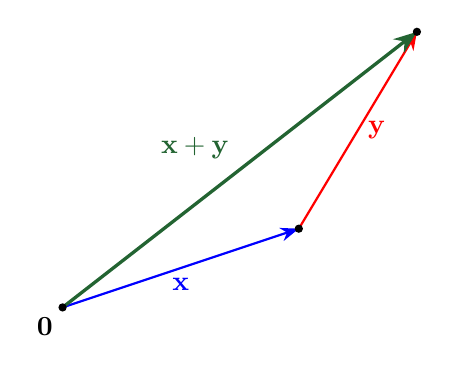
\begin{tikzpicture}[scale=1.0]
    % Vectors
    \coordinate (O) at (0,0);
    \coordinate (X) at (3,1);
    \coordinate (XY) at (4.5,3.5);

    % x vector
    \draw[-{Stealth}, thick, blue] (O) -- (X)
      node[midway, below] {$\mathbf{x}$};
    % y vector from tip of x
    \draw[-{Stealth}, thick, red] (X) -- (XY)
      node[midway, right] {$\mathbf{y}$};
    % x+y vector
    \draw[-{Stealth}, thick, proofcolor, line width=1.2pt] (O) -- (XY)
      node[midway, above left] {$\mathbf{x} + \mathbf{y}$};

    % Origin
    \fill (O) circle (1.5pt);
    \node[below left] at (O) {$\mathbf{0}$};
    \fill (X) circle (1.5pt);
    \fill (XY) circle (1.5pt);
  \end{tikzpicture}
  \end{center}
  \vspace{-0.5em}
  \[
    |\mathbf{x}+\mathbf{y}| \leq |\mathbf{x}| + |\mathbf{y}|
  \]

  \note{
    This diagram illustrates the triangle inequality in "R" 2. The vector "x"
    is shown in blue, the vector "y" in red, and their sum "x" plus "y" in
    green. The three vectors form a triangle. The triangle inequality says
    that the length of the green side --- the direct route from the origin to
    the tip of "x" plus "y" --- is at most the sum of the lengths of the blue
    and red sides. The shortcut is never longer than the detour. Now let's
    prove these properties.
  }
\end{frame}

% =============================================================================
% PROOF OF THEOREM 1.37
% =============================================================================

\section{Proof of Theorem 1.37}

\begin{frame}{Proof Strategy: Theorem 1.37}
  \textbf{Goal:} Prove all six properties of the norm.

  \vspace{0.8em}
  \textbf{Approach:}
  \begin{enumerate}
    \item Parts (a), (b), (c): follow directly from the definition
    \item Part (d): immediate from the \alert{Schwarz inequality} (Theorem 1.35)
    \item Part (e): expand $|\mathbf{x}+\mathbf{y}|^2$ and apply (d)
    \item Part (f): follows from (e) by substitution
  \end{enumerate}

  \note{
    Before diving in, let's outline the strategy. Parts "a", "b", and "c"
    are obvious from the definition of the norm, so we won't spend much time
    on them. Part "d", the Schwarz inequality, was essentially proved in the
    previous section. The real work is in part "e", the triangle inequality,
    which requires us to expand a squared norm and apply the Schwarz
    inequality. Part "f" then follows from "e" by a clever substitution.
    Let's go through each part.
  }
\end{frame}

\begin{frame}{Proof of Parts (a), (b), and (c)}
  \begin{proofblock}{Parts (a), (b), (c)}
    Recall $|\mathbf{x}| = \bigl(\sum_{i=1}^k x_i^2\bigr)^{1/2}$.

    \vspace{0.3em}
    \textbf{(a)} Each $x_i^2 \geq 0$, so $|\mathbf{x}| \geq 0$.

    \vspace{0.2em}
    \textbf{(b)} $|\mathbf{x}| = 0 \;\Leftrightarrow\; \sum x_i^2 = 0
      \;\Leftrightarrow\; \text{each } x_i = 0
      \;\Leftrightarrow\; \mathbf{x} = \mathbf{0}$.

    \vspace{0.2em}
    \textbf{(c)} $|\alpha\mathbf{x}|
      = \bigl(\sum (\alpha x_i)^2\bigr)^{1/2}
      = \bigl(\alpha^2 \sum x_i^2\bigr)^{1/2}
      = |\alpha|\,|\mathbf{x}|$.
  \end{proofblock}

  \note{
    These three parts are straightforward. Part "a" holds because each
    "x" "i" squared is nonnegative, so the sum is nonnegative, and the square
    root of a nonnegative number is nonnegative. Part "b" says the norm is
    zero exactly when all coordinates are zero, which is clear because a sum
    of squares of real numbers is zero only when each term is zero. Part "c"
    uses the fact that alpha squared factors out of the sum and then out of
    the square root, becoming the absolute value of alpha. Now let's handle
    the more interesting parts.
  }
\end{frame}

\begin{frame}{Proof of Part (d): Schwarz Inequality}
  \begin{proofblock}{Part (d): $|\mathbf{x} \cdot \mathbf{y}| \leq |\mathbf{x}|\,|\mathbf{y}|$}
    This is an \alert{immediate consequence} of the Schwarz inequality
    (Theorem~1.35), which was proved in the previous section for sums of the form
    \[
      \left|\sum a_j \bar{b}_j\right|^2
        \leq \sum |a_j|^2 \cdot \sum |b_j|^2.
    \]
    For real numbers, $\bar{b}_j = b_j$ and $|a_j|^2 = a_j^2$, giving exactly:
    \[
      |\mathbf{x} \cdot \mathbf{y}|^2 \leq |\mathbf{x}|^2 \cdot |\mathbf{y}|^2.
    \]
  \end{proofblock}

  \note{
    Part "d" does not require any new work. In the previous section on the
    complex field, we proved the Schwarz inequality for sums involving complex
    numbers. Since real numbers are a special case of complex numbers, where
    the conjugate of "b" "j" is just "b" "j" itself, the Schwarz inequality
    applies directly. Taking square roots of both sides gives us the result.
    Now let's prove the triangle inequality, which is where the Schwarz
    inequality gets used in a beautiful way.
  }
\end{frame}

% --- Proof of (e): progressive build ---
% --- Step 1: Expand ---
\begin{frame}{Proof of Part (e): Triangle Inequality --- Step 1}
  \begin{proofblock}{Step 1: Expand $|\mathbf{x}+\mathbf{y}|^2$}
    \begin{align*}
      |\mathbf{x} + \mathbf{y}|^2
        &= (\mathbf{x}+\mathbf{y}) \cdot (\mathbf{x}+\mathbf{y}) \\
        &= \mathbf{x}\cdot\mathbf{x} + 2\,\mathbf{x}\cdot\mathbf{y}
          + \mathbf{y}\cdot\mathbf{y} \\
        &= |\mathbf{x}|^2 + 2\,\mathbf{x}\cdot\mathbf{y} + |\mathbf{y}|^2
    \end{align*}
  \end{proofblock}

  \note{
    Here is the key computation. We compute the squared norm of "x" plus "y"
    by expanding it using the definition of the inner product. The inner
    product distributes over addition just like ordinary multiplication,
    giving us three terms. The middle term, 2 times the inner product of "x"
    and "y", is the cross term that we need to estimate. Let's apply the
    Schwarz inequality to it.
  }
\end{frame}

% --- Step 2: Apply Schwarz ---
\begin{frame}{Proof of Part (e): Triangle Inequality --- Step 2}
  \begin{proofblock}{Step 2: Apply the Schwarz inequality}
    By part (d): $\;\mathbf{x}\cdot\mathbf{y} \leq |\mathbf{x}\cdot\mathbf{y}|
      \leq |\mathbf{x}|\,|\mathbf{y}|$.

    \vspace{0.3em}
    Therefore:
    \begin{align*}
      |\mathbf{x} + \mathbf{y}|^2
        &\leq |\mathbf{x}|^2 + 2\,|\mathbf{x}|\,|\mathbf{y}| + |\mathbf{y}|^2 \\
        &= \bigl(|\mathbf{x}| + |\mathbf{y}|\bigr)^2
    \end{align*}

    \vspace{0.3em}
    Taking square roots:
    $\;\boxed{|\mathbf{x} + \mathbf{y}| \leq |\mathbf{x}| + |\mathbf{y}|}$
  \end{proofblock}

  \note{
    The Schwarz inequality tells us that the cross term "x" dot "y" is at most
    the product of the norms. Substituting this bound into our expansion, the
    right-hand side becomes a perfect square. Taking square roots of both
    sides completes the proof of part "e". Notice how elegant this is: the
    entire triangle inequality proof comes down to a single application of the
    Schwarz inequality to the cross term. Now let's finish with part "f".
  }
\end{frame}

\begin{frame}{Proof of Part (f): Distance Form}
  \begin{proofblock}{Part (f): Substitution trick}
    In part (e), replace $\mathbf{x}$ with $\mathbf{x} - \mathbf{y}$ and
    $\mathbf{y}$ with $\mathbf{y} - \mathbf{z}$:

    \vspace{0.3em}
    \[
      |(\mathbf{x}-\mathbf{y}) + (\mathbf{y}-\mathbf{z})|
        \leq |\mathbf{x}-\mathbf{y}| + |\mathbf{y}-\mathbf{z}|
    \]

    \vspace{0.3em}
    The left side simplifies:
    $\;(\mathbf{x}-\mathbf{y})+(\mathbf{y}-\mathbf{z}) = \mathbf{x}-\mathbf{z}$.

    \vspace{0.3em}
    Therefore:
    $\;\boxed{|\mathbf{x} - \mathbf{z}| \leq |\mathbf{x} - \mathbf{y}|
      + |\mathbf{y} - \mathbf{z}|}$
    \hfill $\square$
  \end{proofblock}

  \note{
    Part "f" is a direct consequence of part "e". We make the substitution:
    replace "x" with "x" minus "y", and replace "y" with "y" minus "z". On
    the left side, the "y" terms cancel, giving "x" minus "z". So we get the
    distance form of the triangle inequality. This version says the distance
    from "x" to "z" is at most the distance from "x" to "y" plus the distance
    from "y" to "z". This is exactly the property needed to make "R" "k" a
    metric space, as we will see in Chapter 2. That completes the proof of
    Theorem 1.37.
  }
\end{frame}

% =============================================================================
% REMARK 1.38
% =============================================================================

\section{Remarks}

% --- Build 1/3 ---
\begin{frame}{Remark 1.38}
  \begin{remblock}{Remark 1.38}
    Theorem 1.37 parts (a), (b), and (f) show that $\mathbb{R}^k$ can be regarded
    as a \alert{metric space}, with distance $d(\mathbf{x}, \mathbf{y}) = |\mathbf{x} - \mathbf{y}|$.
  \end{remblock}

  \note{
    Remark 1.38 makes the important observation that properties "a", "b", and
    "f" are exactly the axioms for a metric space, which we will define
    formally in Chapter 2. The function that sends two points "x" and "y" to
    the norm of "x" minus "y" gives a well-defined notion of distance. This
    distance is nonnegative, is zero only when the two points coincide, and
    satisfies the triangle inequality. Let's note the special cases.
  }
\end{frame}

% --- Build 2/3 ---
\begin{frame}{Remark 1.38}
  \begin{remblock}{Remark 1.38}
    Theorem 1.37 parts (a), (b), and (f) show that $\mathbb{R}^k$ can be regarded
    as a \alert{metric space}, with distance $d(\mathbf{x}, \mathbf{y}) = |\mathbf{x} - \mathbf{y}|$.
  \end{remblock}

  \vspace{0.5em}
  \textbf{Special cases:}
  \begin{itemize}
    \item $\mathbb{R}^1$ = the \emph{real line}; the norm is the absolute value $|x|$
  \end{itemize}

  \note{
    When "k" equals 1, the space "R" 1 is just the set of all real numbers,
    also known as the real line. The norm of a one-tuple containing "x" is
    just the square root of "x" squared, which is the absolute value of "x".
    So the norm in "R" 1 is exactly the absolute value we have been using all
    along. Now let's look at the two-dimensional case.
  }
\end{frame}

% --- Build 3/3 ---
\begin{frame}{Remark 1.38}
  \begin{remblock}{Remark 1.38}
    Theorem 1.37 parts (a), (b), and (f) show that $\mathbb{R}^k$ can be regarded
    as a \alert{metric space}, with distance $d(\mathbf{x}, \mathbf{y}) = |\mathbf{x} - \mathbf{y}|$.
  \end{remblock}

  \vspace{0.5em}
  \textbf{Special cases:}
  \begin{itemize}
    \item $\mathbb{R}^1$ = the \emph{real line}; the norm is the absolute value $|x|$
    \item $\mathbb{R}^2$ = the \emph{plane} (= the \emph{complex plane}); the norm is the
      modulus $|z|$
  \end{itemize}

  \note{
    When "k" equals 2, the space "R" 2 is the plane. Rudin notes that we can
    identify "R" 2 with the complex plane by comparing Definitions 1.24 and
    1.36: match the pair "a", "b" with the complex number "a" plus "b" "i".
    Under this identification, the norm of the pair "a", "b" is the square
    root of "a" squared plus "b" squared, which is exactly the modulus of the
    corresponding complex number. So the Euclidean norm on "R" 2 and the
    complex modulus are the same thing. This unifies the real, complex, and
    higher-dimensional settings under one framework. Let's wrap up with a
    summary.
  }
\end{frame}

% =============================================================================
% SUMMARY
% =============================================================================

\section{Summary}

% --- Build 1/4 ---
\begin{frame}{Summary}
  \textbf{Key takeaways from this section:}
  \begin{itemize}
    \item $\mathbb{R}^k$ is the set of ordered $k$-tuples; a \alert{vector space} over $\mathbb{R}$
  \end{itemize}

  \note{
    Let's review what we covered. We began by defining "R" "k" as the set of
    all ordered "k"-tuples of real numbers, with component-wise addition and
    scalar multiplication making it a vector space over the real field. But
    a vector space alone is not enough for analysis.
  }
\end{frame}

% --- Build 2/4 ---
\begin{frame}{Summary}
  \textbf{Key takeaways from this section:}
  \begin{itemize}
    \item $\mathbb{R}^k$ is the set of ordered $k$-tuples; a \alert{vector space} over $\mathbb{R}$
    \item The \alert{inner product} $\mathbf{x}\cdot\mathbf{y} = \sum x_i y_i$
      and \alert{norm} $|\mathbf{x}| = (\mathbf{x}\cdot\mathbf{x})^{1/2}$ give
      $\mathbb{R}^k$ its geometry
  \end{itemize}

  \note{
    We then introduced the inner product and the norm, which give "R" "k" its
    geometric structure. The inner product captures the idea of angle, and the
    norm captures the idea of length. These are the tools we need to measure
    things in "R" "k".
  }
\end{frame}

% --- Build 3/4 ---
\begin{frame}{Summary}
  \textbf{Key takeaways from this section:}
  \begin{itemize}
    \item $\mathbb{R}^k$ is the set of ordered $k$-tuples; a \alert{vector space} over $\mathbb{R}$
    \item The \alert{inner product} $\mathbf{x}\cdot\mathbf{y} = \sum x_i y_i$
      and \alert{norm} $|\mathbf{x}| = (\mathbf{x}\cdot\mathbf{x})^{1/2}$ give
      $\mathbb{R}^k$ its geometry
    \item The \alert{Schwarz inequality} and \alert{triangle inequality}
      (Theorem 1.37) are the key results
  \end{itemize}

  \note{
    The main results are the Schwarz inequality and the triangle inequality.
    The Schwarz inequality bounds the inner product by the product of norms,
    and the triangle inequality bounds the norm of a sum by the sum of norms.
    Together, these make "R" "k" a well-behaved geometric space. And the
    payoff is our final takeaway.
  }
\end{frame}

% --- Build 4/4 ---
\begin{frame}{Summary}
  \textbf{Key takeaways from this section:}
  \begin{itemize}
    \item $\mathbb{R}^k$ is the set of ordered $k$-tuples; a \alert{vector space} over $\mathbb{R}$
    \item The \alert{inner product} $\mathbf{x}\cdot\mathbf{y} = \sum x_i y_i$
      and \alert{norm} $|\mathbf{x}| = (\mathbf{x}\cdot\mathbf{x})^{1/2}$ give
      $\mathbb{R}^k$ its geometry
    \item The \alert{Schwarz inequality} and \alert{triangle inequality}
      (Theorem 1.37) are the key results
    \item $\mathbb{R}^k$ is a \alert{metric space}, unifying $\mathbb{R}^1$, $\mathbb{R}^2 \cong \mathbb{C}$,
      and higher dimensions
  \end{itemize}

  \vspace{0.5em}
  \textbf{Coming up next:} The Appendix --- constructing $\mathbb{R}$ from $\mathbb{Q}$
  via Dedekind cuts.

  \note{
    Finally, we saw that "R" "k" is a metric space, with distance defined by
    the norm. This unifies the real line, the complex plane, and all
    higher-dimensional Euclidean spaces under a single framework. This
    framework is exactly what we need to do topology and analysis in multiple
    dimensions, which begins in Chapter 2. In the next and final section of
    Chapter 1, we look at the Appendix, where Rudin constructs the real
    numbers from the rationals using Dedekind cuts. Thank you for watching.
  }
\end{frame}

\end{document}
